% SNU Dissertation for CUMG members v1.2
% Modified for Department of Physics and Astronomy
%%%%%%%%%%%%%%%%%%%%%%%%%%%%%%%%%%%%%%%%%%%%%%%%%%%%%%%%%%%%%%%%
%% v.1.2 RELEASE NOTE
% Margins: adjusted text height (bottom margin) to allow for proper space for page number when printed
% Colophone page: inserted the SNU seal 
% Chapter style: consistent chapter style applied to abstract and acknowledgements
% Reduced flexibility for paragraph spacing (\addtolength{\parskip}{0pt plus 3pt minus 3pt})
% Title page: English title page adjusted
% Additional notes on bibliography style
%%%%%%%%%%%%%%%%%%%%%%%%%%%%%%%%%%%%%%%%%%%%%%%%%%%%%%%%%%%%%%%%
%% v1.1 RELEASE NOTE
% fixed typos, colophone margin and website address bug
% variable page number box for table of contents
% fixed inconsistent styles btw thm and def
% Hardcover (Eng. ver.) redesign
%%%%%%%%%%%%%%%%%%%%%%%%%%%%%%%%%%%%%%%%%%%%%%%%%%%%%%%%%%%%%%%%
% LaTeX template designed by zeta709 and heavily modified by S. Moon
% For printing on A4 paper, use ``fit'' option
% For submission copy, consider turning on all entries under (ssss)
% For defense manuscript, turn on the defense cover (dddd) and turn off all others (ssss)
% Be sure to modify ./Injun/injun (인준지) and references.bib (인용)
% For questions, please do not hesistate: sj.moon.math@gmail.com

%%%%%%%%%%%%%%%%%%%%%%%%%%%%%%%%%%%%%%%%%%%%%%%%%%%%%%%%%%%%%%%%
%% UNDER THE HOOD (DO NOT MODIFY IF YOU DON'T KNOW WHAT YOU'RE DOING)
%%%%%%%%%%%%%%%%%%%%%%%%%%%%%%%%%%%%%%%%%%%%%%%%%%%%%%%%%%%%%%%%
\RequirePackage{fix-cm}
% options
% 	oneside
% 	twoside
% 	ko: Korean
% 	master
% 	phd
% 	openright: chapter title only on odd pages
\documentclass[twoside,phd,4x6]{snuthesis}

%%%%%%%%%%%%%%%%%%%%%%%%%%%%%%%%%%%%%%%%%%%%%%%%%%%%%%%%%%%%%%%%%%%%%%%%%%%%%%
%%
%% Author: zeta709 (zeta709@gmail.com)
%% Releasedate: 2017/07/20
%%
%% 목차 양식을 변경하는 코드
%% * subfigure (subfig) package 사용 여부에 따라
%%   tocloft의 옵션을 다르게 지정해야 한다.
%% * Chapter 번호가 두 자리 수를 넘어가는 경우 다음과 같이
%%   필요한 만큼 "9"를 추가하면 된다.
%%   \settowidth{\mytmplen}{\bfseries\cftchappresnum9\cftchapaftersnum}
%%   아니면 \cftchapnumwidth를 직접 적당히 고치면 된다.
%%%%%%%%%%%%%%%%%%%%%%%%%%%%%%%%%%%%%%%%%%%%%%%%%%%%%%%%%%%%%%%%%%%%%%%%%%%%%%
%\usepackage[titles,subfigure]{tocloft} % when you use subfigure package
\usepackage[titles]{tocloft} % when you don't use subfigure package
\makeatletter
\if@snu@ko
	\renewcommand\cftchappresnum{제~}
	\renewcommand\cftchapaftersnum{~장}
	\renewcommand\cftfigpresnum{그림~}
	\renewcommand\cfttabpresnum{표~}
\else
	\renewcommand\cftchappresnum{}
	\renewcommand\cftfigpresnum{}
	\renewcommand\cfttabpresnum{}
\fi
\makeatother
\newlength{\mytmplen}
\settowidth{\mytmplen}{\bfseries\cftchappresnum\cftchapaftersnum}
\addtolength{\cftchapnumwidth}{\mytmplen}
\settowidth{\mytmplen}{\bfseries\cftfigpresnum\cftfigaftersnum}
\addtolength{\cftfignumwidth}{\mytmplen}
\settowidth{\mytmplen}{\bfseries\cfttabpresnum\cfttabaftersnum}
\addtolength{\cfttabnumwidth}{\mytmplen}
\makeatletter
\g@addto@macro\appendix{%
	\addtocontents{toc}{%
		\settowidth{\mytmplen}{\bfseries\protect\cftchappresnum\protect\cftchapaftersnum}%
		\addtolength{\cftchapnumwidth}{-\mytmplen}%
		\protect\renewcommand{\protect\cftchappresnum}{\appendixname~}%
		\protect\renewcommand{\protect\cftchapaftersnum}{}%
		\settowidth{\mytmplen}{\bfseries\protect\cftchappresnum\protect\cftchapaftersnum}%
		\addtolength{\cftchapnumwidth}{\mytmplen}%
	}%
}
\makeatother
 % SNU toc style
\newlength\longest

%% PDF SET UP
\ifpdf
	\input glyphtounicode\pdfgentounicode=1 %type 1 font
	\usepackage[pdftex]{graphicx}
\else
	\usepackage[dvipdfmx]{graphicx}
\fi


\renewcommand{\cftpartpresnum}{Part~}
\let\cftoldpartfont\cftpartfont
\renewcommand{\cftpartfont}{\cftoldpartfont\cftpartpresnum} %part in front of part number
\cftpagenumbersoff{part} % page number off for parts


\usepackage[defaultlines=2,all]{nowidow} % do you hate poor widows?
% \usepackage{lipsum} % lorem ipsum example contents
\usepackage{xpatch}
\usepackage{booktabs} % to use \toprule \midrule \bottomrule commands in tabular
\usepackage[backend=bibtex,style=phys,biblabel=brackets,maxbibnames=12,maxcitenames=2,sortcites=false,url=false,doi=false]{biblatex}
	\setlength\bibitemsep{\baselineskip} % spacing between bibitems when single-spacing is used
	\addtolength\bibitemsep{0pt plus 10pt minus 10pt} % some wiggle room for bibitem spacing
	% \xpatchbibmacro{date}{%
	% 	\printtext[parens]%
	% }{%
	% 	\setunit*{\addcomma\space}%
	% 	\printtext%
	% }{}{} 
	% \renewbibmacro{in:}{}
	% \DeclareFieldFormat[article,incollection,inproceedings]{pages}{#1}
	% \DeclareFieldFormat[book,inbook]{pages}{#1\addspace pp\adddot} % pp. for books
	% \DeclareDelimFormat[bib,biblist]{nametitledelim}{\addcolon\space} % colon after year
	% \DeclareFieldFormat
	% [article,incollection,inproceedings]
	% {title}{#1}
	% \renewbibmacro*{journal+issuetitle}{%
	% 	\usebibmacro{journal}%
	% 	\setunit*{\addcomma\space}%
	% 	\iffieldundef{series}
	% 	{}
	% 	{\newunit
	% 		\printfield{series}%
	% 		\setunit{\addspace}}%
	% 	\usebibmacro{volume+number}%
	% 	\setunit{\addspace}%
	% 	\usebibmacro{issue+date}%
	% 	\setunit{\addcolon\space}%
	% 	\usebibmacro{issue}%
	% 	\newunit}
	% \DeclareFieldFormat{journaltitle}{\mkbibemph{#1\isdot}}
	% \DeclareFieldFormat[article]{volume}{\bfseries #1}
	% \renewbibmacro{volume+number}{% removing number entry
	% 	\printfield{volume}}
	% \DeclareFieldFormat{titlecase}{\MakeTitleCase{#1}}
	% \newrobustcmd{\MakeTitleCase}[1]{%
	% 	\ifthenelse{\ifcurrentfield{booktitle}\OR\ifcurrentfield{booksubtitle}%
	% 	\OR\ifcurrentfield{maintitle}\OR\ifcurrentfield{mainsubtitle}%
	% 	\OR\ifcurrentfield{journaltitle}\OR\ifcurrentfield{journalsubtitle}%
	% 	\OR\ifcurrentfield{issuetitle}\OR\ifcurrentfield{issuesubtitle}%
	% 	\OR\ifentrytype{book}\OR\ifentrytype{mvbook}\OR\ifentrytype{bookinbook}%
	% 	\OR\ifentrytype{booklet}\OR\ifentrytype{suppbook}%
	% 	\OR\ifentrytype{collection}\OR\ifentrytype{mvcollection}%
	% 	\OR\ifentrytype{suppcollection}\OR\ifentrytype{manual}%
	% 	\OR\ifentrytype{periodical}\OR\ifentrytype{suppperiodical}%
	% 	\OR\ifentrytype{proceedings}\OR\ifentrytype{mvproceedings}%
	% 	\OR\ifentrytype{reference}\OR\ifentrytype{mvreference}%
	% 	\OR\ifentrytype{report}\OR\ifentrytype{thesis}}
	% 	{#1}
	% 	{\MakeSentenceCase{#1}}} % make only first letter of article title capital only
	\addbibresource{references.bib}
	% comma after author even when there are two authors (AMS peculiarity)
	% \AtBeginBibliography{%
	% 	\renewcommand*{\finalnamedelim}{%
	% 	%   \ifnumgreater{\value{liststop}}{2}{\finalandcomma}{} % removed from original
	% 		\finalandcomma % added to original
	% 		\addspace\bibstring{and}\space}%
	% 	}


\usepackage{amsmath} \allowdisplaybreaks[4] % this will allow page breaks for align. Likelihood options: 0-4
% \usepackage{amssymb}
% \usepackage{amsthm}
% %	\theoremstyle{definition}
% 	\newtheoremstyle{newdef}% name of the style to be used
% 	{}% measure of space to leave above the theorem. E.g.: 3pt
% 	{}% measure of space to leave below the theorem. E.g.: 3pt
% 	{}% name of font to use in the body of the theorem
% 	{}% measure of space to indent
% 	{\bfseries}% name of head font
% 	{}% punctuation between head and body
% 	{1em}% space after theorem head; " " = normal interword space
% 	{}
% 	\theoremstyle{newdef}
% 	\newtheorem{definition}{Definition}[chapter]
% 	\makeatletter
% 	\def\thm@space@setup{%
% 		\thm@preskip=0.5\baselineskip % modifying buffer for theorems and definitions
% 		\thm@postskip=\thm@preskip % or whatever, if you don't want them to be equal
% 	}
% 	\makeatother
% 	\newtheoremstyle{slthm}% name of the style to be used
% 	{}% measure of space to leave above the theorem. E.g.: 3pt
% 	{}% measure of space to leave below the theorem. E.g.: 3pt
% 	{\slshape}% name of font to use in the body of the theorem
% 	{}% measure of space to indent
% 	{\bfseries}% name of head font
% 	{}% punctuation between head and body
% 	{1em}% space after theorem head; " " = normal interword space
% 	{}
% 	\theoremstyle{slthm}
% 	\newtheorem{theorem}{Theorem}[chapter]
% 	\newtheorem{corollary}{Corollary}[theorem]
% 	\newtheorem{lemma}[theorem]{Lemma}
% 	\newtheorem{proposition}{Proposition}[chapter]
\usepackage{commath}
\renewcommand{\labelenumi}{\upshape{(\alph{enumi})}}
\renewcommand{\labelenumii}{\alph{enumi}~\Roman{enumii}.}
\usepackage{enumitem}
	\setlist{nolistsep} % remove spacing between items in a list
\usepackage{upgreek}
\usepackage{mathrsfs}
\usepackage{siunitx}
\usepackage[dvipsnames]{xcolor}
\usepackage{tikz}
\usetikzlibrary{positioning}
\tikzset{>=latex}
\usepackage{tabularx}
\usepackage[flushleft]{threeparttable}
%\usepackage{kbordermatrix} % http://www.hss.caltech.edu/~kcb/TeX/kbordermatrix.sty
%	\renewcommand{\kbldelim}{[} % Left delimiter
%	\renewcommand{\kbrdelim}{]} % Right delimiter
%	\newcommand\scalemath[2]{\scalebox{#1}{\mbox{\ensuremath{\displaystyle #2}}}} % matrix scaling
\usepackage[nodisplayskipstretch]{setspace} 
% remove setspace package to change back caption spacing to double spacing & delete font= options below
% setspace option also meant to reduce display equation spacing
\usepackage[labelfont=bf]{caption} % change number for spacing modification in: font={stretch=1.1}
	\captionsetup[figure]{labelfont={bf},name={Figure},labelsep=quad,font={stretch=1.1}}
	\captionsetup[table]{labelfont={bf},name={Table},labelsep=quad,font={stretch=1.1}}
\usepackage{tocloft} % table of contents
	\setlength\cftbeforesubsecskip{0.5\baselineskip} % item spacing for toc subsections - if single spacing used
	\setlength\cftbeforesecskip{0.5\baselineskip} % item spacing for toc sections - if single spacing is used
	\setlength\cftbeforechapskip{\baselineskip} % item spacing for toc chapters - if single spacing is used
	\setlength\cftbeforefigskip{\baselineskip} % item spacing for list of figures - if single spacing used
	\setlength\cftbeforetabskip{\baselineskip} % item spacing for list of tables - if single spacing used
	\addtolength\cftbeforefigskip{0pt plus 10pt minus 10pt} % wiggle room for figure spacing
	\addtolength\cftbeforetabskip{0pt plus 10pt minus 10pt} % wiggle room for table spacing
	\renewcommand{\cftchapdotsep}{\cftnodots} % change to 2 if leader dots for chap are desired
	\renewcommand{\cftsecdotsep}{2}
	\renewcommand{\cftsubsecdotsep}{2}
	\renewcommand{\cftfigdotsep}{2}
	\renewcommand{\cfttabdotsep}{2} % adjust number to control spacing between the dots
	\renewcommand{\cftpnumalign}{r} % l: page number left-aligned, r: page number right-aligned
% remove spacing between chapters in lof and lot
\usepackage{xpatch}

\makeatletter
\xpatchcmd{\@chapter}{%
	\addtocontents{lof}{\protect\addvspace{10\p@}}%
	\addtocontents{lot}{\protect\addvspace{10\p@}}%
}{}{}{}
\makeatother
%\usepackage[T1]{fontenc}
%\usepackage[utf8]{inputenc}
\usepackage{etoolbox}
	\AtBeginEnvironment{quote}{\singlespace\vspace{-\topsep}}
	\AtEndEnvironment{quote}{\vspace{-\topsep}\endsinglespace}
\usepackage[activate={true,nocompatibility},final,tracking=true,kerning=true,spacing=true,factor=1100,stretch=10,shrink=10]{microtype}
	\SetTracking{encoding={*}, shape=sc}{40} % reduce spacing in scshape
	\hyphenpenalty=1500 % reduce hyphenation frequency (10000 to disallow it completely)
%	\exhyphenpenalty=100 % allows preexisting hyphens 
%	\pretolerance=2000 % allowing some white spaces (9999 to maximize)
%	\tolerance=2000 % allowing some white spaces (9999 to maximize) TeX's secondattempt
\setlength{\skip\footins}{2\baselineskip} % proper spacing between footnote and main text
%\counterwithout{footnote}{chapter} % continuous numbering of footnotes throughout doc if desired
\usepackage{mathtools} % for dashed and dotted lines %\sampleline{},\sampleline{dashed},\sampleline{dotted},\sampleline{dash pattern=on .7em off .2em on .05em off .2em}
\DeclareRobustCommand\sampleline[1]{%
	\tikz\draw[#1,line width=0.35mm] (0,0) (0,\the\dimexpr\fontdimen22\textfont2\relax)
	-- (1.5em,\the\dimexpr\fontdimen22\textfont2\relax);%
}
\usepackage[figuresright]{rotating}
%\renewcommand{\arraystretch}{0.75}
\raggedbottom % removes random spacing between paragraphs, use with caution! To undo, use \flushbottom
\usepackage{imakeidx}
	\makeindex[columns=2, title=Index, 
	options= -s mystyle.ist]
	% get rid of unwanted indent
	\makeatletter
	\def\@idxitem{\par\hangindent 0pt}
	\makeatother
	\indexsetup{othercode=\small}
	
\usepackage{lettrine}
\usepackage{GoudyIn}
\renewcommand{\LettrineFontHook}{\color{black}\GoudyInfamily{}}
	\setcounter{DefaultLines}{3}
	\setlength{\DefaultNindent}{0pt}
	\setlength{\DefaultFindent}{1pt}
	\usepackage{pgfornament}
	
\usepackage{needspace} % for unusual circumstances requiring more space in page (ex. \needspace{4\baselineskip})

\usepackage{titlesec}
\titleformat{\section}{\normalfont\fontsize{14}{14}\bfseries}{\thesection}{1em}{\hspace{0em}}{}
\titleformat{\chapter}{\normalfont\fontsize{16}{16}\bfseries}{\thechapter}{1em}{\hspace{0em}}{}

\usepackage{afterpage} % needed for full page figures
\makeatletter
\@fpsep\textheight
\afterpage{\global\setlength\@fpsep{8\p@ \@plus 2fil}}
\makeatother

\renewcommand\floatpagefraction{.001}
\makeatletter
\setlength\@fpsep{\textheight}
\makeatother

%%%%%%%%%%%%%%%%%%%%%%%%%%%%%%%%%%%%%%%%%%%%%%%%%%%%%%%%%%%%%%%%%%
%% END OF UNDER THE HOOD
%%%%%%%%%%%%%%%%%%%%%%%%%%%%%%%%%%%%%%%%%%%%%%%%%%%%%%%%%%%%%%%%%%

%%%%%%%%%%%%%%%%%%%%%%%%%%%%%%%%%%%%%%%%%%%%%%%%%%%%%%%%%%%%%%%%%%
%% USER-DEFINED MACROS (ADD YOUR OWN AS NEEDED)
%%%%%%%%%%%%%%%%%%%%%%%%%%%%%%%%%%%%%%%%%%%%%%%%%%%%%%%%%%%%%%%%%%
\newcommand{\ihat}{\hat{\textbf{\i}}} % tensor notation stuff
\newcommand{\jhat}{\hat{\textbf{\j}}}
\newcommand{\khat}{\mathbf{\hat{k}}}
\let\oldvec\vec 
\renewcommand{\vec}[1]{\mathbf{#1}}
\newcommand{\ddt}[2]{\frac{\Delta {#1}}{\Delta{#2}}}
\newcommand{\pdt}[2]{\frac{\partial #1}{\partial #2}}
\newcommand{\paren}[1]{\left( #1 \right)}
\def \nobreakseq {\nobreak \hskip 0pt \hbox}
%\def\v#1{\vec{#1}}

%%%%%%%%%%%%%%%%%%%%%%%%%%%%%%%%%%%%%%%%%%%%%%%%%%%%%%%%%%%%%%%%%%
%% USER INFORMATION
%%%%%%%%%%%%%%%%%%%%%%%%%%%%%%%%%%%%%%%%%%%%%%%%%%%%%%%%%%%%%%%%%%

%% TITLE
\title{The renormalization group and short distance behavior in non-Abelian gauge theory} % main title
\title*{비-아벨리안 게이지 이론에서의 재규격화 군과 짧은 거리 성질} % Korean title

%% 소속
\academicko{이학}
\schoolen{서울대학교 대학원}
\departmenten{물리천문학부 물리학전공}
\departmentko{물리천문학부 물리학전공}
% \bachelors{Jibang University}
% \bsyear{2013}
% \masters{Waeguk University}
% \msyear{2016}

%% Author's(Your) name
\author{Choonkyu Lee} % English Name
\author*{이~~준~~규} % Korean Name

%% 학번
\studentnumber{1975-12345}

%% 지도교수님 성함 Advisor's name
\advisor{Choonkyu Lee}
\advisor*{이~준~규}

%% 학위 수여일 Graduation date
\graddate{2024년~~2월} % Graduation Year and Month in Korean
\endate{February 2024} % Graduation Month in English

%% Note: 인준지의 교수님 성함은
%% 컴퓨터로 출력하지 않고, 교수님께서
%% 자필로 쓰시기도 합니다.

%% Committee members' names in Korean
\committeemembers%
{임~지~순}%
{이~준~규}%
{박~제~근}%
{김~기~훈}%
{김~석}%

%% Committee members' names in English
\encommitteemembers%
{Professor Jisoon Ihm, Chair}%
{Professor Choonkyu Lee, Advisor}%
{Professor Park, Je-Geun}%
{Professor Kee Hoon Kim}%
{Professor Seok Kim}%


\authorallcaps{CHOONKYU LEE} % All caps English name
% \cvlink{www.yourwebsite.com} % link to your CV or personal website

%% 학위 수여일 Graduation date
\defensedate{1975년~~1월~~1일} % Defense Date in Korean
\gradyear{1976} % Year of Graduation

%% PDF Information
\usepackage[]{hyperref}
\hypersetup{
	pdftitle={Choonkyu Lee PhD Dissertation},
	pdfauthor={Choonkyu Lee},
	pdfsubject={PhD Dissertation},
	pdfkeywords={SNU},
	bookmarksnumbered=true,     
	bookmarksopen=true,         
	bookmarksopenlevel=1,       
	colorlinks=false, % do not use links for references and footnotes
	hidelinks, % remove ugly boxed windows indicating links           
	pdfstartview=Fit, % choose "Fit" to start with fit window            
	pdfpagemode=UseOutlines,    % outlines on pdf document
	pdfpagelayout=TwoPageRight % two page viewer with odd number pages to the right/ other option: "OneColumn" for scrolling
}

\usepackage{pdfpages} % activate for inserting injun.pdf
%\renewcommand{\theequation}{\thechapter.\arabic{equation}} % chapter 0 considerations
%\renewcommand{\thefigure}{\thechapter.\arabic{figure}} % chapter 0 considerations

\usepackage{mypackages}

\begin{document}
\pagenumbering{Roman}


%%%%%%%%%%%%%%%%%%%%%%%%%%%%%%%%%%%%%%%%%%%%%%%%%%%%%%%%%%%%%%%
%% FRONT MATTER
%%%%%%%%%%%%%%%%%%%%%%%%%%%%%%%%%%%%%%%%%%%%%%%%%%%%%%%%%%%%%%%

%% Cover to be used for thesis defense (dddd)
%\presentation{최종} % options: 최종, 중간, 제안
%\makefrontcover % final defence

%% Hardcover (English version) (ssss)
%\hardcoveren
%\cleardoublepage

% Hardcover (Default - Korean based) (ssss)
\hardcover
\cleardoublepage

%% To Insert Injun Page (ssss)
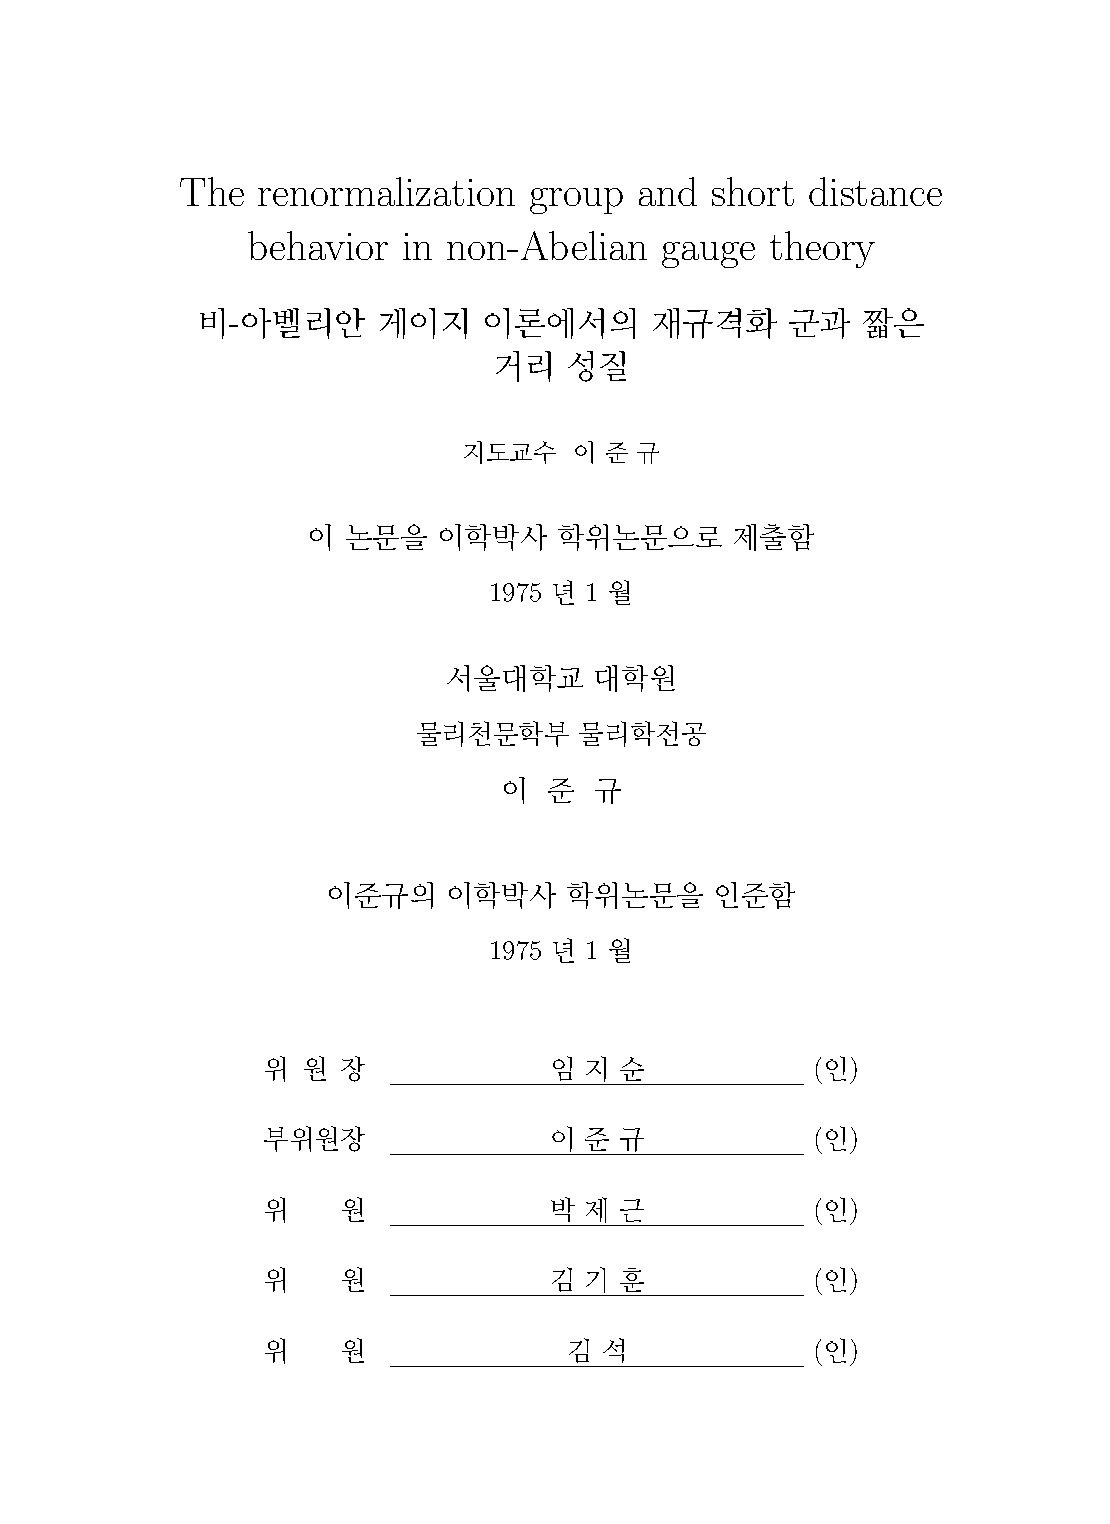
\includepdf[pages=-]{./injun.pdf} % injun template in FinalDraft2 folter
\cleardoublepage

%% Turn on inner cover (English title and committee member names) options: jadae vs. non-jadae (ssss)
%\makefrontcoveren % for those who did not go to snu for undergrand and master's
\makefrontcoverenjadae % jadae option for those who went to snu for undergrand


%% REQUIRED
\makeapproval % for some reason page margins get messed up without this command


%% Colophon (ssss)
\publications{Name~et~al., 2021. \emph{J. Good Sci.} 96, 105708; }{Name~et~al., 2021. \emph{Int. J. Nice Sci.} 31, To Appear; }{}{}{}
% \makecolophon
% \clearpage
\clearpage\null

%% Dedication page (ssss)
%\thispagestyle{empty}
%\null\vfill
%\settowidth\longest{\lettrine{A}{nte mare et terr\={a}s} et quod tegit omnia caelum}
%\begin{center}
%	\parbox{\longest}{%
%		\raggedleft
%		{\slshape To My Mother}
%	}
%\end{center}
%\vfill\vfill
%\cleardoublepage

%% To Include an epigraph (ssss)
%\cleardoublepage
%\thispagestyle{empty}
%\null\vfill
%\settowidth\longest{\lettrine{A}{nte mare et terr\={a}s} et quod tegit omnia caelum}
%\begin{center}
%	\parbox{\longest}{%
%		\begingroup
%		\setstretch{1.2}
%		\raggedright{%
%			\lettrine{N}{ice} and inspirational quote can be inserted here.\par\bigskip
%		}
%		\raggedleft{---Famous Person, \emph{Magnum Opus}}\par%
%		\endgroup
%	}
%\end{center}
%\vfill\vfill
%\cleardoublepage

%%%%%%%%%%%%%%%%%%%%%%%%%%%%%%%%%%%%%%%%%%%%%%%%%%%%%%%%%%%%%%%%%%%%
%% ABSTRACT
%%%%%%%%%%%%%%%%%%%%%%%%%%%%%%%%%%%%%%%%%%%%%%%%%%%%%%%%%%%%%%%%%%%%
\pagenumbering{roman} % start page numbering (first in Roman numeral)

\keyword{Non-Abelian gauge theory, renormalization group}
\begin{abstract}
\noindent

My abstract

My abstract

My abstract
\end{abstract}

%% Turn on for acknowledgmentin the front matter (English)
%\cleardoublepage
%\acknowledgment
%Thank you.
\clearpage

%%%%%%%%%%%%%%%%%%%%%%%%%%%%%%%%%%%%%%%%%%%%%%%%%%%%%%%%%%%%%%%%%%%%%%%%%%%
%% TABLE OF CONTENTS, LIST OF FIGURES, ETC (NO NEED TO MODIFY; ALREADY FORMATTED)
%%%%%%%%%%%%%%%%%%%%%%%%%%%%%%%%%%%%%%%%%%%%%%%%%%%%%%%%%%%%%%%%%%%%%%%%%%%
\begingroup
\setstretch{1.1} % make multiline chapter titles single spaced, also turn on tocloft options
	\cftsetpnumwidth{2.0em} \cftsetrmarg{3.55em} % adjust spacing between page number and title
	\phantomsection\clearpage\addcontentsline{toc}{chapter}{Contents}%
%	\tableofcontents
	{\def\makebox[#1][#2]#3{#3}\tableofcontents}
\endgroup
% some tolerance for nicer pagenation
\addtolength{\topskip}{0pt plus 5pt minus 5pt}
\addtolength{\parskip}{0pt plus 3pt minus 3pt}
% make captions single spacing in list of figures and list of tables
% be sure to also modify tocloft options for item separation
\begin{sloppypar} % sloppy command here to avoid overfull hbox
\begingroup
\emergencystretch 1em % reduce spacing between words under sloppy
\countdef\interlinepenalty255 %allow pagebreaks for LoF figure captions
\setstretch{1.1} 
	\cftsetpnumwidth{2.0em} \cftsetrmarg{3.55em} % adjust spacing between page number and caption
	\clearpage\phantomsection\clearpage\addcontentsline{toc}{chapter}{List of Figures}%
%	\listoffigures
    {\def\makebox[#1][#2]#3{#3}\listoffigures}
	\clearpage\phantomsection\clearpage\addcontentsline{toc}{chapter}{List of Tables}%
%	\listoftables
    {\def\makebox[#1][#2]#3{#3}\listoftables}
\endgroup
\end{sloppypar}

\flushbottom % For consistent bottom page margins, use with caution! to undo, use \raggedbottom
\addtolength{\baselineskip}{0pt plus 1pt minus 1pt} % with flushbottom, give linespace some room

\cleardoublepage % fresh start for chapter 1
\pagenumbering{arabic}
\addtolength{\topskip}{0pt plus-3pt minus-3pt} %undo too much wiggle room
\addtolength{\parskip}{0pt plus-4pt minus-4pt}
%\setcounter{chapter}{-1} % Chapter 0 for "Overview" (per tradition).

%%%%%%%%%%%%%%%%%%%%%%%%%%%%%%%%%%%%%%%%%%%%%%%%%%%%%%%%%%%%%%%%%%%%%%%%%%%%%%%%%
%% MAIN CONTENTS (START WRITING YOUR DISSERTATION!)
%%%%%%%%%%%%%%%%%%%%%%%%%%%%%%%%%%%%%%%%%%%%%%%%%%%%%%%%%%%%%%%%%%%%%%%%%%%%%%%%%

\chapter[Introduction]{Introduction} \label{ch:1_intro}

We elaborate on both field-theoretic and quantum mechanical descriptions of (non-)Abelian anyons, emphasizing the role of contact interaction terms. Field theoretic contact terms, required for the sake of renormalizability in general, implement the self-adjoint extension of the quantum mechanical Hamiltonian~\cite{Lee1997}.



\begin{figure}[tb]
\centering

\includegraphics[width=0.6\linewidth]{figures/mechanics.jpg}
\caption[Essential Classical Mechanics]{
	This is a book on intermediate classical mechanics.
	In this book, classical mechanics is presented as a useful tool to analyze the physical universe and also as the base on which the whole pyramid of modern physics has been erected. 
	Various mechanical concepts are developed in a highly logical manner, with relatively thorough treatments on mathematical procedures and many physically interesting applications. 
	Connections to more modern theoretical developments (including statistical physics, relativity, and quantum mechanics) are emphasized~\cite{Lee2018Book}.
}
\label{fig:plph_GaAs}
\end{figure}

% \input{chapter2.tex}

% \input{chapter3.tex}

% ...


%%%%%%%%%%%%%%%%%%%%%%%%%%%%%%%%%%%%%%%%%%%%%%%%%%%%%%%%%%%%%%%%%%%%
%% END OF MAIN MATTER
%%%%%%%%%%%%%%%%%%%%%%%%%%%%%%%%%%%%%%%%%%%%%%%%%%%%%%%%%%%%%%%%%%%%

%%%%%%%%%%%%%%%%%%%%%%%%%%%%%%%%%%%%%%%%%%%%%%%%%%%%%%%%%%%%%%%%%%%%
%% BACK MATTER
%%%%%%%%%%%%%%%%%%%%%%%%%%%%%%%%%%%%%%%%%%%%%%%%%%%%%%%%%%%%%%%%%%%%

%% BIBLIOGRAPHY
\clearpage
\begingroup
    \setstretch{1.1} % remove to make all references double spacing 
    % (remember to remove \setlength\bibitemsep in preamble if you choose to use double spacing)
    %\nohyphenation % turn on to prevent hyphenation in bibliography
	\phantomsection\clearpage\addcontentsline{toc}{chapter}{Bibliography}
	\printbibliography
\endgroup

%% Turn on for acknowledgment (English) (ssss)
%\cleardoublepage
%\acknowledgment
%Thank you!
%
%{\raggedleft \hspace*{\fill}Your Name\\\hspace*{\fill}Seoul, July 2030}

%% Turn on to include index (ssss)
%\cleardoublepage
%\begingroup
%\setstretch{1.2}
%\phantomsection\clearpage\addcontentsline{toc}{chapter}{Index}
%\printindex
%\endgroup

%% Turn on for Korean abstract (ssss)
\cleardoublepage
%\addtolength{\topskip}{0pt plus-10pt}
%\addtolength{\parskip}{0pt plus-10pt}
% !compose Korean abstract separately and copy--paste. Many TeX editors do not play well with Korean typing!
% need to manually indent at the start of the first paragraph (Korean writing)
\keywordalt{비-아벨리안 게이지 이론, 재규격화 군}
\begin{abstractalt}
\hspace{\parindent}
초록은 동색이다.
이 말은 풀색과 녹색은 같은 색이라는 뜻으로 같은 처지에 있는 사람들끼리 같이 어울리게 마련이라는 생각을 담고 있다.
초색과 녹색을 합하여 초록이라 하듯이 서로 같은 무리끼리 잘 어울린다는 의미로 사용되고 있다.
\end{abstractalt}

%% Turn on for Korean acknowledgment (ssss)
% \cleardoublepage
% \acknowledgement
% \hspace{\parindent}한국어로 감사합니다!

\end{document}
